ss[12pt,a4paper]{article}
\usepackage[utf8]{inputenc}
\usepackage{natbib}
\usepackage{graphicx}
\usepackage{float}
\setcounter{secnumdepth}{5}
\setcounter{tocdepth}{4}
\usepackage{tabularx}

\usepackage{multirow}
\usepackage{framed}
\begin{document}
\begin{center}

 \vspace*{1cm}
  \LARGE
  \textbf{Projet POCA\\}
  \large
 
   \large
  	\vspace{2cm}
  \textbf{Université Paris Diderot- Master 2}\\
  \vspace{1cm}
  \LARGE
  \textbf{Thème}\\

  \LARGE
  \setlength{\fboxsep}{0.5cm}
  \begin{framed}
	\textbf{Role play game over internet}
  \end{framed}
  \vspace{2cm}
\begin{table}[H]
   \setlength{\tabcolsep}{2cm}
    \large
	\centering
	\begin{tabular}{l}
		\textbf{Réalisé par :}    
		 \\  \\
		 -\textbf{ Achachour} Hamza\\
		-\textbf{ Baghor} Soufiane\\
	
	-\textbf{ Douihech } Maha \\
		-\textbf{ Kebaili} Zohra Kaouter \\
		-\textbf{ Mouhoubi } Khawla \\
		
  

	\end{tabular}
  \end{table}
  \vspace{\fill}
  \large
  \textbf{Promotion 2018/2019}
   \end{center}
\title{\Huge{Analyse des besoins}}

\date{Version 1: 15 octobre 2018}
\newpage




\section{Description du logiciel}
\par Le logiciel à réaliser dans ce projet est une plateforme permettant de créer et participer à des jeux de rôle en ligne où le maître du jeu et les personnages joueurs communiquent via un chat.

\section{Requis fonctionnels}
Un requis fonctionnel exprime comment est le
système du point de vue utilisateur. Nous rappelons que notre projet est destiné principalement à être utilisé par des joueurs en rôle. Nous recensons donc ce qui suit les Requis fonctionnels de notre système que nous avons séparé en 3 modules :
\begin{itemize}
	\item Connexion \& Inscription
	\item Jeux de rôle. 
	\item Actions. 

\end{itemize}
Ces requis sont prioritisés comme suit:\\
\begin{center}
	\begin{table}[H]
		\centering
		\begin{tabular}{ll}
			\textbf{Priorité} & \textbf{Description}                                               \\
			M (Must have)   & \begin{tabular}[c]{@{}l@{}}Spécification obligatoire et fondamentale.
			\end{tabular}          \\
			S (Should have)  & \begin{tabular}[c]{@{}l@{}}Spécification importante mais non fondamentale.\end{tabular} \\
			C (Could have)  & Spécification optionnelle mais non fondamentale.                           
			\\
			W (Want to have) & \begin{tabular}[c]{@{}l@{}}Spécification non importante.\end{tabular}
		\end{tabular}\\
		\caption{Priorités de spécifications Méthode MoSCoW.}
		\label{moscow}
	\end{table}
\end{center}
L'effort est mis en nombre de jours nécessaires de réalisation.
\begin{table}[H]
	\centering
	
	\begin{tabular}{|l|l|p{8cm}|l|l|}
		\hline
		ID &Module& Requis&Priorité& Effort \\ 
		\hline
		US1 & \multirow{3}{*}{\begin{tabular}[c]{@{}l@{}}Connexion \\ \& Inscription\end{tabular}} &S'inscrire pour utiliser les fonctionnalités offertes par la plateforme.& M & 5 \\ \cline{1-1} \cline{3-4} \cline{4-5}
		US2 &  &L'utilisateur inscrit peut se connecter à une session. & M&5 \\ \cline{1-1} \cline{3-4} \cline{4-5}
		US3 &  & Rejeter un joueur qui rejoint si la capacité du jeu est dépassée. & M&5 \\\hline 
	
		US4 & \multirow {3}{*} {Jeux de rôle }&Créer un nouveau jeu de rôle en spécifiant son nom, son scénario et ses personnages.  & M&5\\\cline{1-1} \cline{3-4} \cline{4-5}
		
		US5 &  & Un joueur personnage peut rejoindre un jeu existant. & M &5\\ \cline{1-1} \cline{3-4} \cline{4-5}
		US6 &  & Le maitre du jeu peut créer une ou plusieurs fiches personnages. & M &5\\ \hline
		US7 & \multirow{7}{*}{ Actions} & Un joueur personnage peut envoyer un message. & M&5 \\ \cline{1-1} \cline{3-4} \cline{4-5}
		US8 &  &Un joueur personnage peut envoyer un message privé à un joueur en particulier. & M &5\\ \cline{1-1} \cline{3-4} \cline{4-5}
		US9 &  &Un joueur personnage peut envoyer un fichier(sonore ou image). & M &5\\ \cline{1-1} \cline{3-4} \cline{4-5}
		US10 &  &  Un joueur personnage peut écrire une commande sur le chat qui simulera un lancer de dé. & M&5 \\\cline{1-1} \cline{3-4} \cline{4-5}
		US11 &  & Le maitre du jeu peut répondre à une action manuellement. & M &5\\ \cline{1-1} \cline{3-4} \cline{4-5}
		US12 &  & Le maitre du jeu peut répondre à une action automatiquement. & M &5\\ \cline{1-1} \cline{3-4} \cline{4-5}
		
		US13 &  &Le maitre du jeu peut ajouter une réponse à la liste des réponses automatiques. & M&5 \\ \hline

	\end{tabular}
	\caption{Les spécifications fonctionnelles de la plateforme}
	\label{specifFonct}
\end{table}
\section{Requis non focntionnels}
Un requis non focntionnels exprime comment est le
système d’un point de vue interne (technique,
technologie,…etc.). A présent, nous recensons les spécifications techniques de notre plateforme dans le tableau ci-dessous:
    \begin{table}[H]
	\centering
	
	\label{specifnonFonct}
	\begin{tabular}{|l | p{14.5cm}| }
		\hline	ID & Requis      \\\hline           
		US2	&Les JDR créés doivent supporter plusieurs centaines de joueurs. \\ \hline
		US3	&Le logiciel devra utiliser un client IRC pour les chats. \\ \hline
		
	\end{tabular}
		\caption{Requis non focntionnels}
\end{table}

% Added by Soufiane in collaboration with Kawther 
\section{La liste des tâches}
Le tableau suivant décrit la liste des tâches élémentaires de notre application.
\begin{itemize}
	\item L'Effort par heure ; 
	\item Priorité de 1 à 3 (Ordre croissant : 1 la plus importante) ;  
	\item Difficulté de 1 à 3 étoiles.
\end{itemize}


% Table of tasks
\begin{table}[H]
	\centering
\begin{tabular}{|l|p{1,7cm}|p{4,5cm}|p{5,5cm}|p{0,5cm}|p{0,5cm}|p{0,5cm}|}
		\hline
		ID &Module& Phase & Tache & P & E & D \\ 
		\hline
		T1 &Connexion et Inscription. &\multirow{3}{*} _S'inscrire pour utiliser les fonctionnalités offertes par la plateforme.& Apprendre le protocole IRC & 1 & 4 & *	\\   \cline{1-1}\cline{4-5}\cline{5-6}\cline{6-7}	
        T2 && 	& L’apprentissage du langage Scala & 1 & 8 & *	\\  \cline{1-1}\cline{4-5}\cline{5-6}\cline{6-7}
        T3 && &  Création du module d’authentification en utilisant le protocole IRC & 1 & 2 & **		
     	\\\hline 
	
	
		T4 &&\multirow{7}{*} _Ouverture d’un salon par la création d’un canal de communication. & Se mettre d’accord sur l’ensemble des commandes & 2 & 1 & **	\\   \cline{1-1}\cline{4-5}\cline{5-6}\cline{6-7}	
		
        T5&& 	& Description des scénarios  & 2& 4& ***	\\ \cline{1-1}\cline{4-5}\cline{5-6}\cline{6-7}
        T6&& 	& Définir les actions automatiques et non automatiques & 2& 3& ***	\\  \cline{1-1}\cline{4-5}\cline{5-6}\cline{6-7}
        T7&& 	& Le choix des critères de satisfaction pour le choix des personnages & 2& 2& **	\\  \cline{1-1}\cline{4-5}\cline{5-6}\cline{6-7}
        T8&& 	& Requêtes (commandes) pour obtenir la liste des jeux en cours & 1& 4& **	\\  \cline{1-1}\cline{4-5}\cline{5-6}\cline{6-7}
        T9&& 	& La commande /join pour rejoindre un Jeu & 1& 3& **	\\  \cline{1-1}\cline{4-5}\cline{5-6}\cline{6-7}
        T10&&   & L’option de validation/de refus du personnage proposé  & 3& 3& *		
	\\\hline 
		T11 & Jeux de rôle &\multirow{4}{*} _Jeu & L’envoie des messages (actions) & 1 & 4& **	\\   \cline{1-1}\cline{4-5}\cline{5-6}\cline{6-7}	
		
    T12&& 	& Lancement du dé (choix de la méthode aléatoire équiprobable)  & 2 & 2& **	\\  \cline{1-1}\cline{4-5}\cline{5-6}\cline{6-7}
    T13&& 	& L’option de validation / de refus de l’action par le maître du jeu  & 2 & 3& **	\\  \cline{1-1}\cline{4-5}\cline{5-6}\cline{6-7}
    T14&& &  L’ajout des décisions du maître du jeu à la table des actions automatiques. & 3 & 7& ***		
	\\\hline 
	
	T15 & &\multirow{2}{*}_Communication entre les membres (IRC)&L’ouverture d’un canal des messages publics & 1 & 4& ***	\\   \cline{1-1}\cline{4-5}\cline{5-6}\cline{6-7}	
		

    T16 && &  Louverture d’un canal de communication privée & 2 & 5& ***		
	\\\hline 
		T17 & &\multirow{2}{*} _Quitter le jeu & La commande /leave par l’un des membres & 2 & 3& *	\\   \cline{1-1}\cline{4-5}\cline{5-6}\cline{6-7}	
		
    T18 && &  La commande /end fin du jeu par le maitre du jeu  & 2 & 4& **		
	\\\hline 
	

	\end{tabular}
	\caption{Les tâches}

\end{table}

% Added by Soufiane 
\section{L'architecture}
Le schéma suivant représente l'architecture de notre application.

\centerline{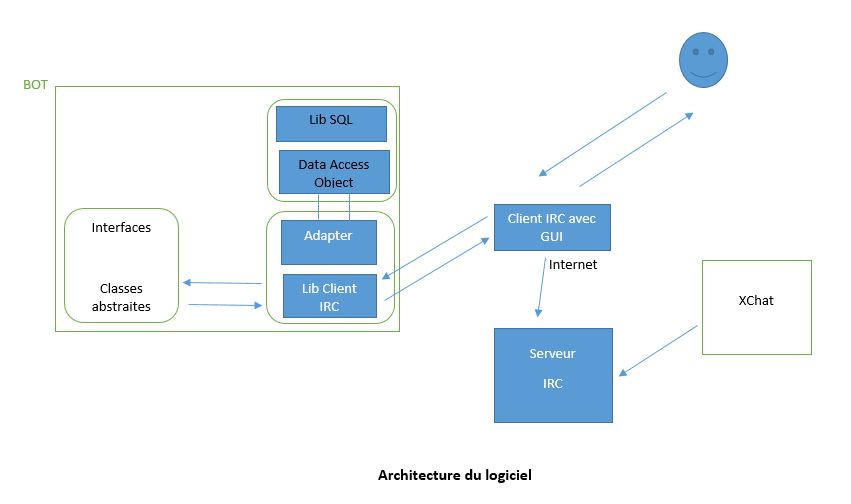
\includegraphics[width=20cm, height=15cm]{Arch.JPG}}


  %  \nocite{*}
  %  \bibliographystyle{apalike} 
	%\renewcommand\bibname{Bibliographie}
%	\bibliography{references}
\end{document}


